\chapter{RESULTS AND DISCUSSION}
\section{Preliminary Results}
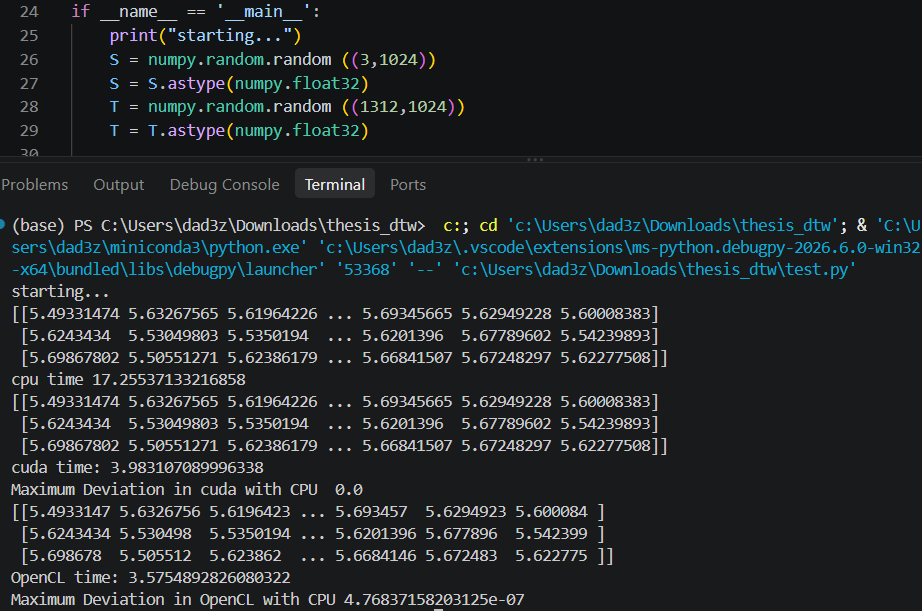
\includegraphics[width=1\linewidth]{prelim1.png}
Figure 4.1: test.py using 3 * 1312

Using a slightly modified version of the provided test.py script from the GPUDTW package, the speed of the CPU to compute DTW can be compared to the speed of the GPU computing DTW using the same inputs. Modifications made include outputing the computed DTW for visual confirmation, removing unnecessary outputs, and lowering the number of data points per sequence due to hardware limitations.

The first array used in testing has 3 sequences with 1024 data points each sequence while the second array has 1312 sequences with 1024 data points each. There are 1024 * 1024 = 1,048,576 cells per pair and 3 * 1312 = 3,936 pairs for a total of 4,127,195,136 cells computed with DTW.

The CPU took an estimated 17.26 seconds while the GPU took an estimated 3.98 seconds through cuda and an estimated 3.58 seconds through OpenCL. Cuda had a 333\% speedup while OpenCl had a 382\% speedup, though cuda no deviation from the CPU's computations while OpenCL's computations match consistently only up to the 6th decimal point. Past the testing stage, only cuda will be used as it is catered towards NVIDIA and to preserve accuracy with results.

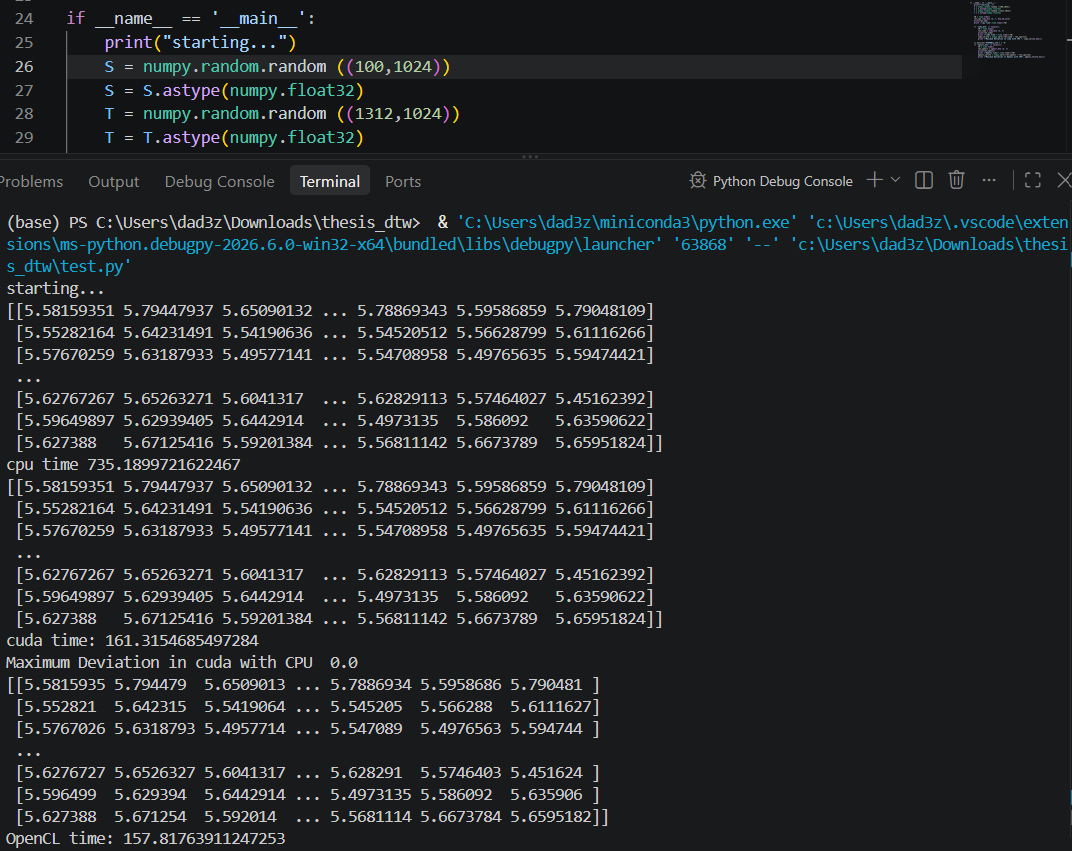
\includegraphics[width=1\linewidth]{prelim2.png}
Figure 4.2: test.py using 100 * 1312

Even with a roughly 33x increase, increasing the amount of cells to be computed to 137,573,171,200 cells, the overall speedup remains relatively consistent with cuda at 355\% speedup and OpenCL at 365\% speedup